% !TEX TS-program = xelatex
\documentclass[aspectratio=169,11pt,professionalfonts]{beamer}

% Theme
\usetheme[numbering=fraction,progressbar=frametitle]{metropolis}
\metroset{block=fill}

% Fonts (XeLaTeX/LuaLaTeX)
\usepackage{fontspec}
\usepackage{unicode-math}
% Main text font per user request
\setmainfont{Fira Code}
\setmonofont{Fira Code}
% Math font for formulas (Fira Code has no math)
\setmathfont{latinmodern-math.otf}

% Language & basic packages
\usepackage[english]{babel}
\usepackage{graphicx}
\usepackage{booktabs}
\usepackage{tabularx}
\usepackage{amsmath,amssymb,mathtools}
\usepackage{xcolor}
\usepackage{csquotes}
\usepackage{bm}

% Graphics search paths (relative to this file)
\graphicspath{{../../pro-default-model/results/}{../../paper/Long_term/}}

% Macros
\newcommand{\E}{\mathbb{E}}
\newcommand{\bbP}{\mathbb{P}}
\newcommand{\Y}{\mathcal{Y}}
\newcommand{\1}{\mathbb{1}}
\DeclareMathOperator{\Lsig}{L}

% Title
\title{Default with Policy\,–\,Randomness Overestimation (PRO)}
\subtitle{Pivoted Pricing, Deleveraging, and a Stability Illusion}
\author{Chen Gao}
\institute{National School of Development, Peking University}
\date{October 15}

% Section page
\setbeamertemplate{section page}{\centering\begin{minipage}{0.9\linewidth}\centering\usebeamerfont{section title}\insertsection\par\end{minipage}}
\AtBeginSection{
  {\setbeamertemplate{footline}{}
  \begin{frame}[plain]\sectionpage\end{frame}}
}

\begin{document}

% Title
\begin{frame}[plain]
  \titlepage
\end{frame}

% Agenda
\begin{frame}{Roadmap}
  \tableofcontents
\end{frame}

% Motivation
\section{Motivation}

\begin{frame}{A Persistent Puzzle}
  \begin{itemize}
    \item Some sovereigns face persistently high spreads despite moderate debt and
          improving fundamentals.
    \item Event evidence (e.g., Argentina’s inflation misreporting) shows spread
          decoupling beyond direct balance-sheet effects.
    \item Standard models struggle to match elevated average premia with lower
          volatility.
    \item This paper: a single pricing operator with a second-moment belief wedge (PRO)
          that \emph{pivots} price/spread schedules.
  \end{itemize}
\end{frame}

\begin{frame}{Argentina: Data Misreporting and Spread Decoupling}
  \begin{columns}[T,onlytextwidth]
    \column{0.5\textwidth}
    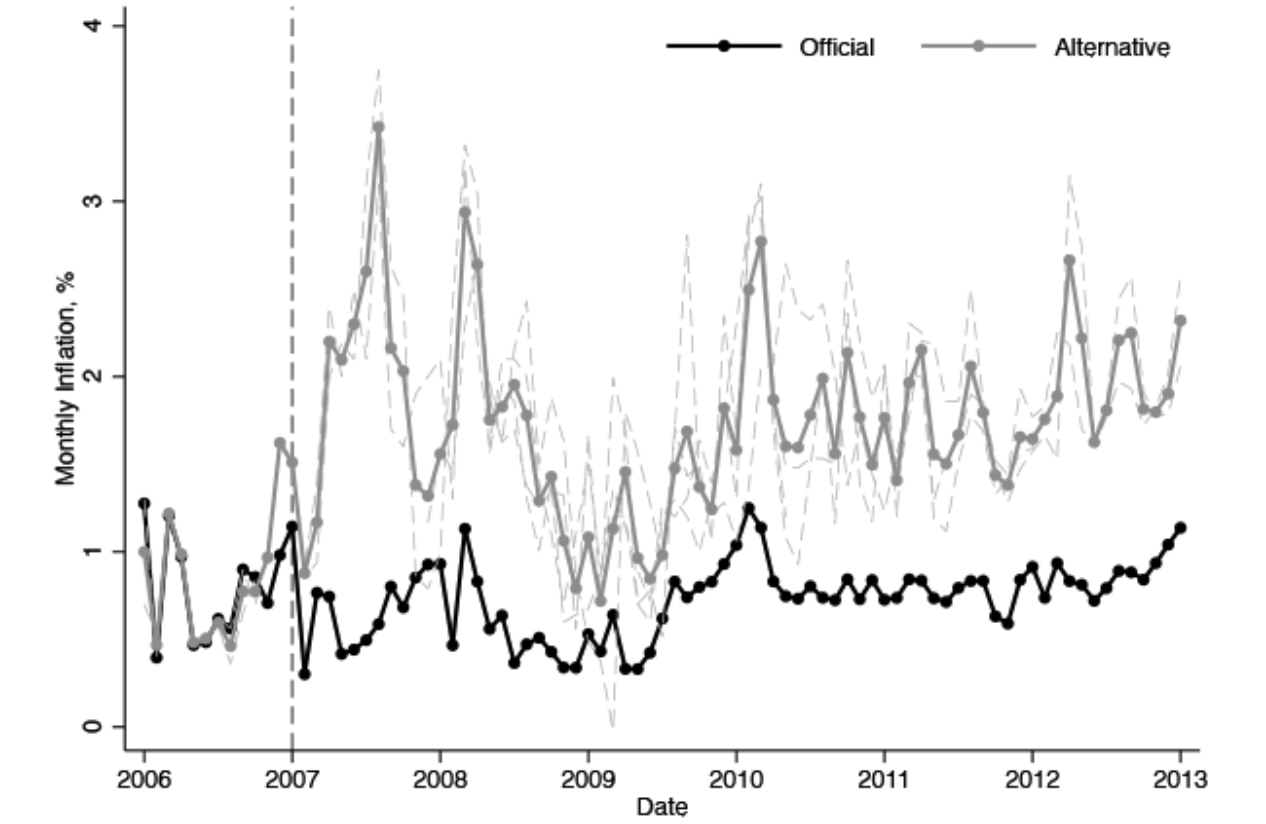
\includegraphics[width=\linewidth]{inflation_arg.png}
    \vspace{0.3em}
    {\scriptsize Official CPI vs. alternative measures}
    \column{0.5\textwidth}
    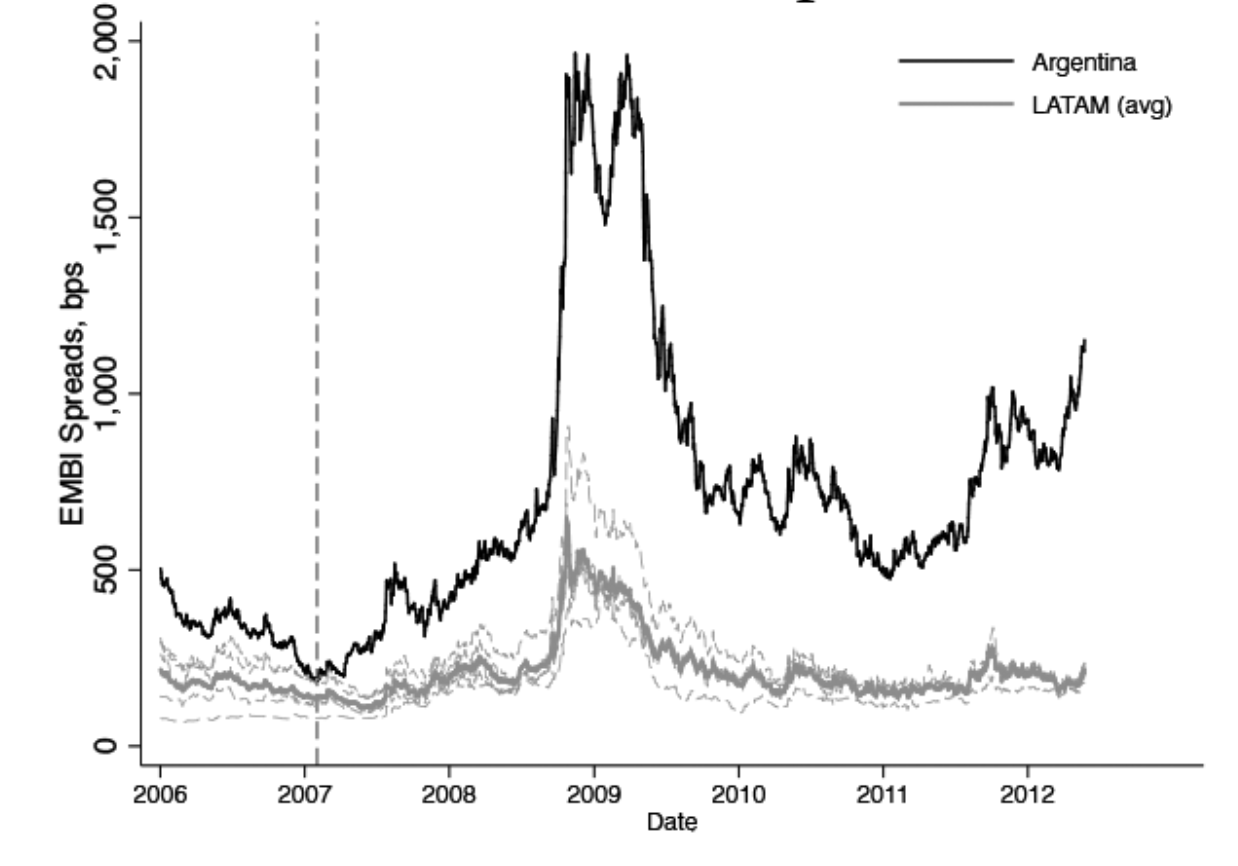
\includegraphics[width=\linewidth]{spread_arg.png}
    \vspace{0.3em}
    {\scriptsize EMBI+ spreads: Argentina vs. LA peers}
  \end{columns}
  \vspace{0.3em}
  \begin{itemize}
    \item Interpretation: reputational channel (type) + PRO (policy dispersion) likely
          both active.
  \end{itemize}
\end{frame}

% Model
\section{Model}

\begin{frame}{Environment}
  \begin{itemize}
    \item Time: $t=0,1,2,\dots$. Endowment $\ln y'=(1-\rho_y)\mu_y+\rho_y\ln
            y+\sigma_y\varepsilon'$, $\varepsilon'\sim\mathcal N(0,1)$.
    \item Long-term debt with coupon $\kappa$, decay $\delta$, risk-free rate $r$.
    \item Default exclusion probability $1-\gamma$; output cost $h(y)=y-\max\{0,\lambda_0
            y+\lambda_1 y^2\}$.
    \item Sovereign utility $u(c)=(c^{1-\sigma}-1)/(1-\sigma)$, discount $\beta$.
  \end{itemize}
\end{frame}

\begin{frame}{Discrete Choice: Default and Borrowing}
  Taste shocks (Gumbel) deliver closed-form aggregator and logit probabilities.
  \begin{align*}
    V(y,B)                & = \eta\,\ln\!\Big( e^{V^D(y)/\eta}+e^{V^R(y,B)/\eta}\Big),                                                         \\
    \bbP\{d{=}1\mid y,B\} & =\frac{e^{V^D(y)/\eta}}{e^{V^D(y)/\eta}+e^{V^R(y,B)/\eta}}\;=\;\Lsig\!\Big(-\tfrac{\Delta V(y,B)}{\eta}\Big),      \\
    V^R(y,B)              & =\rho\,\ln\!\sum_{B'\in\mathcal B} e^{W(y,B,B')/\rho},\quad \bbP\{B'\mid y,B\}=\frac{e^{W/\rho}}{\sum e^{W/\rho}},
  \end{align*}
  where $\Delta V\equiv V^R{-}V^D$, $W(y,B,B')=u\big(y-\kappa B+[B'-(1{-}\delta)B]q(y,B')\big)+\beta\E V(y',B')$.
\end{frame}

\begin{frame}{Lenders and Pricing Operator}
  PRO scales the taste-shock parameter in the \emph{default logit} via a tail weight $\theta\ge1$:
  \begin{equation*}
    P_\theta(y,B')\;=\;\Lsig\!\Big(-\tfrac{\Delta V(y,B')}{\theta\,\eta}\Big),\qquad \Lsig(z)=\tfrac{1}{1+e^{-z}}.
  \end{equation*}
  Pricing operator (unique fixed point):
  \begin{equation*}
    (\mathcal T_\theta q)(B',y)=\frac{1}{1+r}\,\E_{y'|y}\!\Big[(1{-}P_\theta(y',B'))\big(\kappa+(1{-}\delta)\,\E_{B''|y',B'}q(y',B'')\big)\Big].
  \end{equation*}
\end{frame}

% Pivot intuition
\section{Pivot Intuition}

\begin{frame}{One-Line Schematic of Pivot}
  Compact schematic anchoring the single-crossing:
  \begin{align*}
     & P_\theta(y,B')=\Lsig\!\Big(-\tfrac{\Delta V(y,B')}{\theta\eta}\Big),\quad \Delta V\equiv V^R{-}V^D,                                   \\
     & \Rightarrow\quad \mathrm{sign}\big( P_1{-}P_\theta\big)=-\,\mathrm{sign}(\Delta V),                                                   \\
     & \Rightarrow\quad \mathrm{sign}\big(q_\theta{-}q_1\big)=\mathrm{sign}\,\E[(P_1{-}P_\theta)\Pi]\;=\;-\,\mathrm{sign}(\Delta V),\;\Pi>0.
  \end{align*}
  Define the state-dependent threshold $B^*(y):\ \Delta V(y,B^*(y))=0$. Then:
  \begin{itemize}
    \item $B' < B^*(y)$ (safe region, $\Delta V>0$): $\;q_\theta<q_1$ (costlier borrowing).
    \item $B' > B^*(y)$ (near default, $\Delta V<0$): $\;q_\theta>q_1$ (softened doom).
  \end{itemize}
\end{frame}

% Quantitative
\section{Quantitative Results}

\begin{frame}{Calibration (Quarterly, EM stylized)}
  \begin{itemize}
    \item Preferences and endowment: $\sigma=2$, $\beta=0.9775$, $\rho_y=0.95$,
          $\sigma_y=0.005$.
    \item Debt: $\delta=0.04$ (5y duration), $\kappa=\delta{+}r$, $r=1\%$/qtr,
          $\gamma=0.125$.
    \item Default cost: $h(y)=y-\max\{0,\lambda_0 y+\lambda_1 y^2\}$ with
          $(\lambda_0,\lambda_1)=(-0.48,0.525)$.
    \item Taste shocks small: $\eta=5\times10^{-4}$, $\rho=10^{-5}$; grids: $N_y{=}201$,
          $N_B{=}600$.
    \item Scenarios: $\theta\in\{1,10,100\}$.
  \end{itemize}
\end{frame}

\begin{frame}{Business Cycle Moments}
  \begin{columns}[T,onlytextwidth]
    \column{0.56\textwidth}
    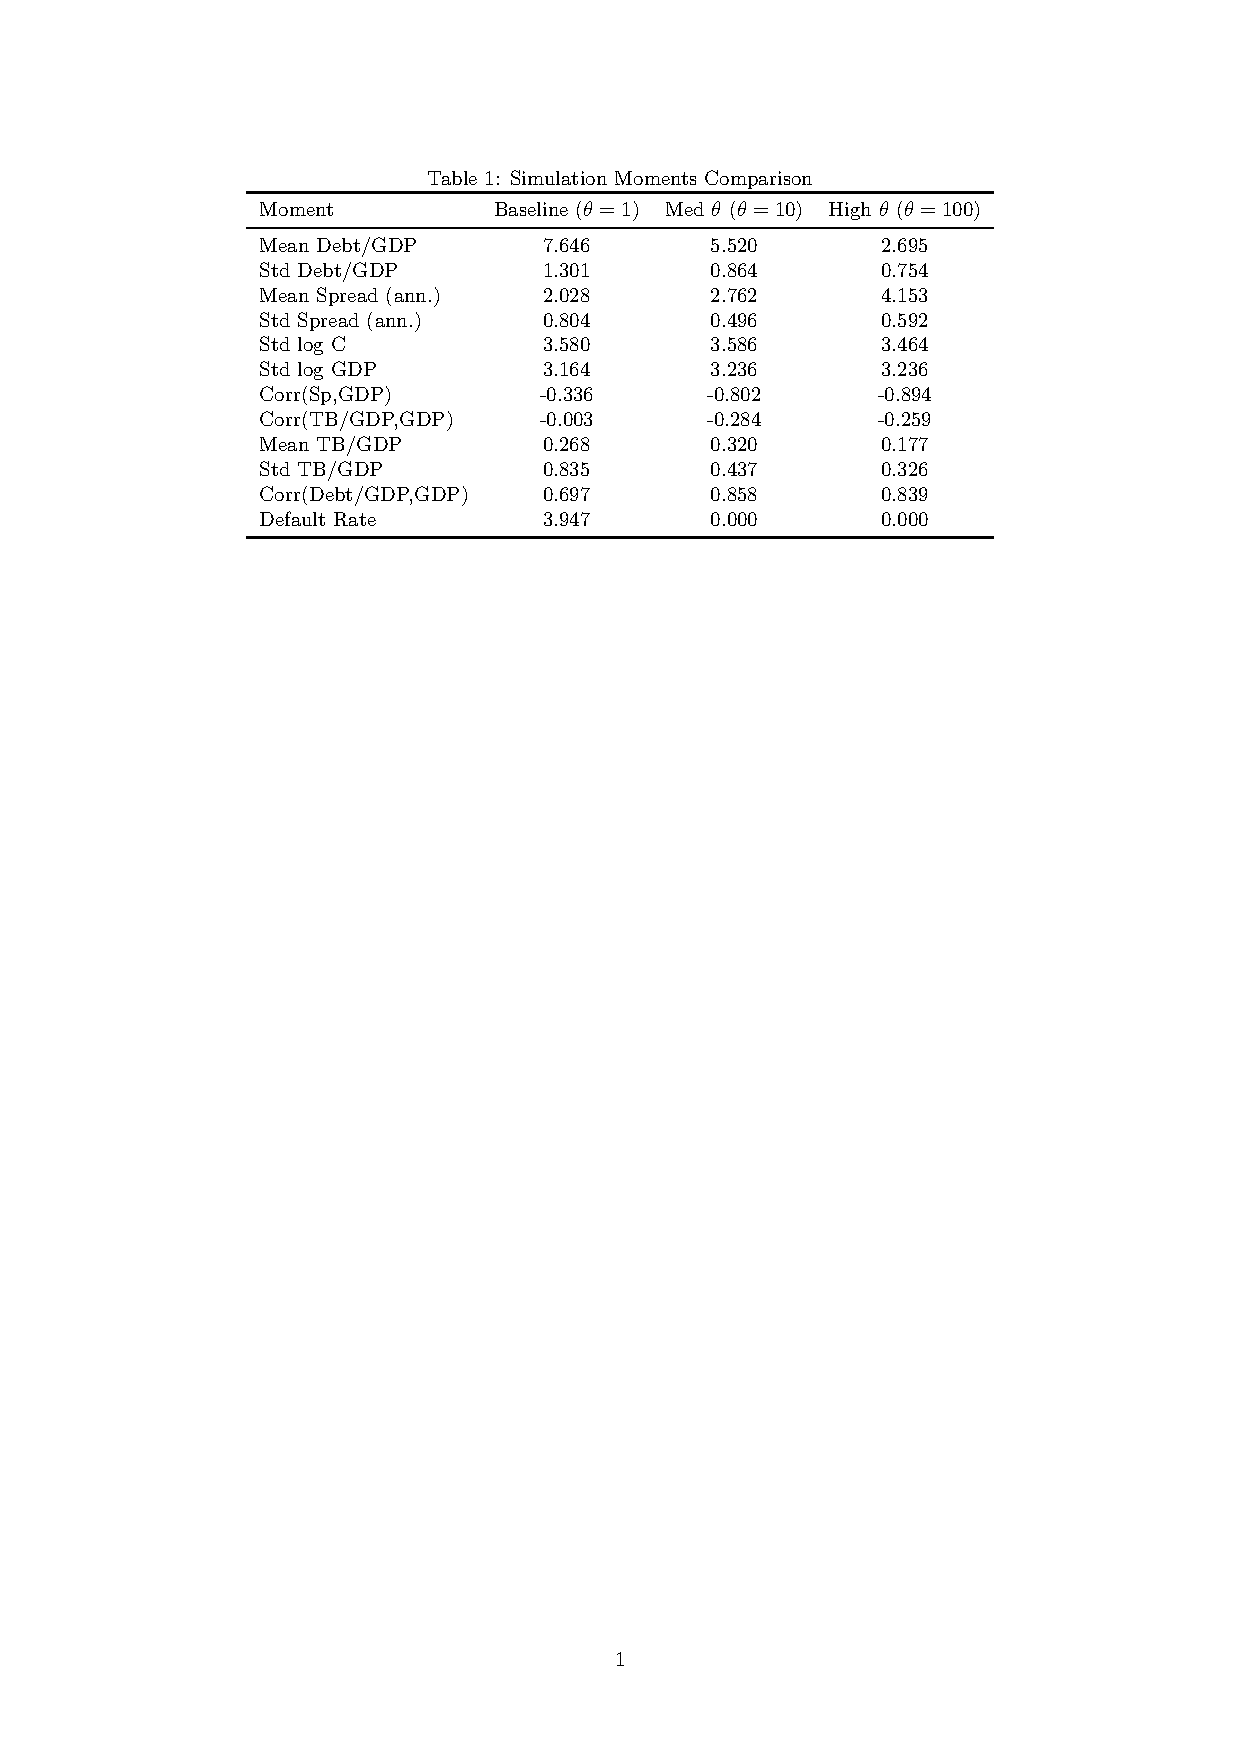
\includegraphics[width=\linewidth]{moments_comparison_table.pdf}
    \column{0.44\textwidth}
    \begin{itemize}
      \item Higher avg spreads with deleveraging (pivot wedge dominates composition).
      \item Spreads more countercyclical; volatility of spreads/debt falls (illusion of
            stability).
      \item Consumption volatility nearly unchanged; risk insurance impaired.
    \end{itemize}
  \end{columns}
\end{frame}

\begin{frame}{Price, Spread, and Default Risk}
  \begin{columns}[T,onlytextwidth]
    \column{0.33\textwidth}
    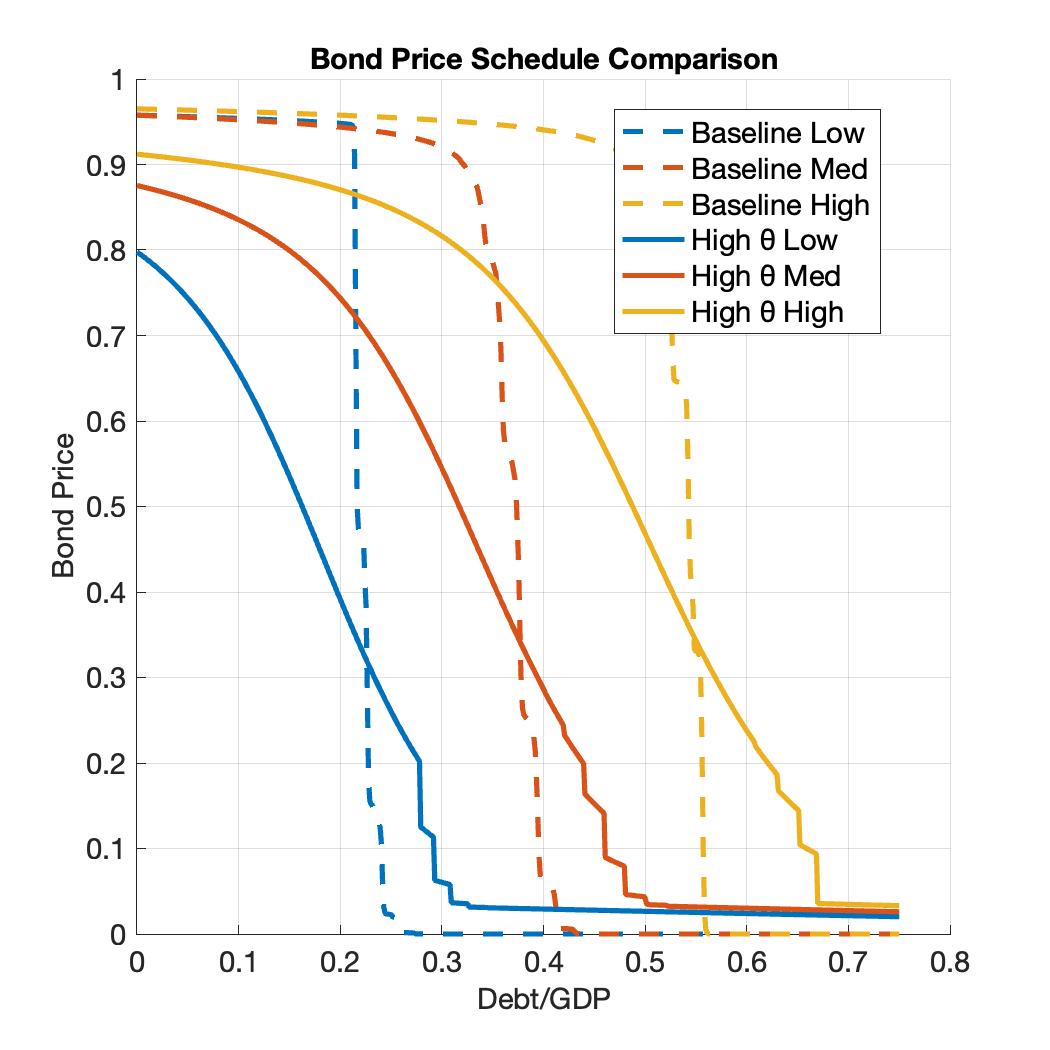
\includegraphics[width=\linewidth]{bond_price_comparison.png}\\[0.3em]
    {\scriptsize Bond prices}
    \column{0.33\textwidth}
    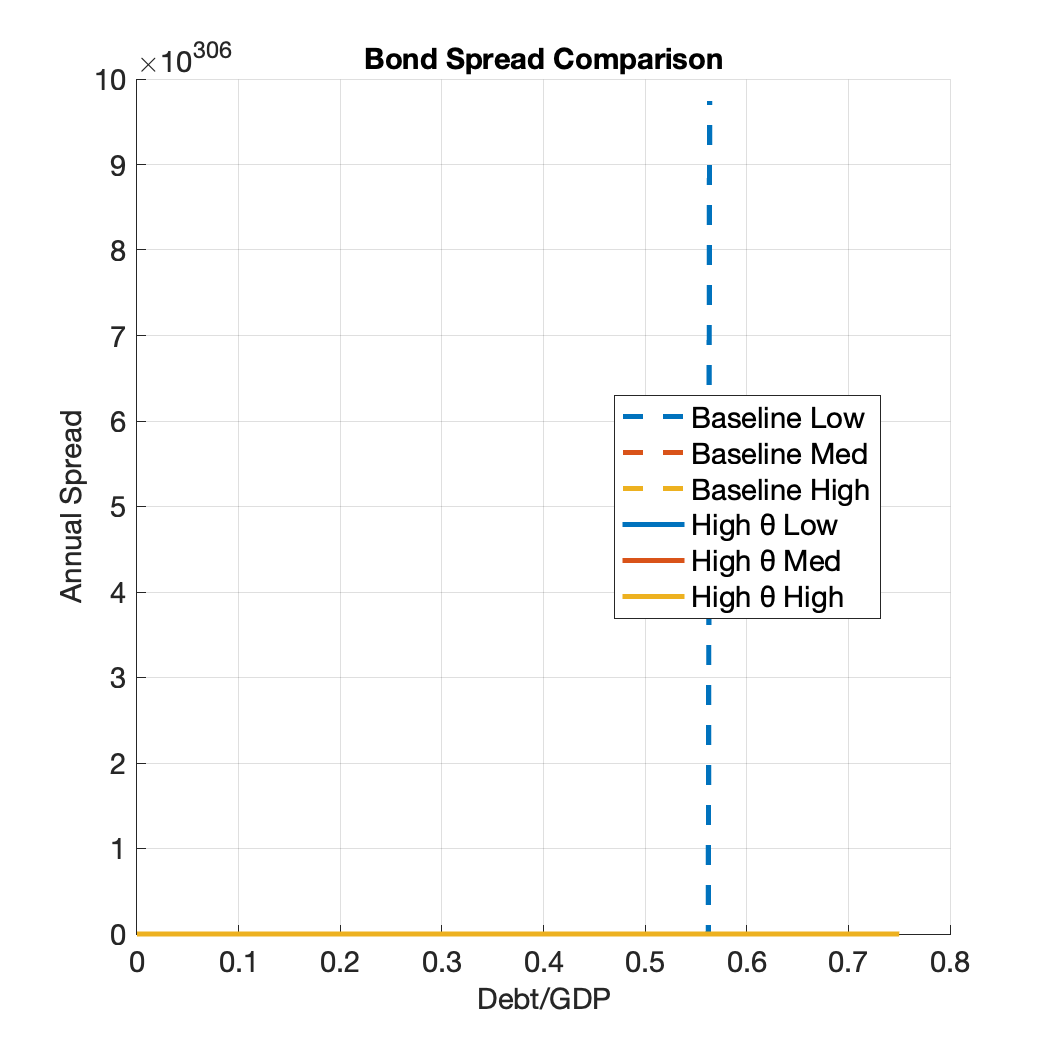
\includegraphics[width=\linewidth]{spread_comparison.png}\\[0.3em]
    {\scriptsize Spreads}
    \column{0.33\textwidth}
    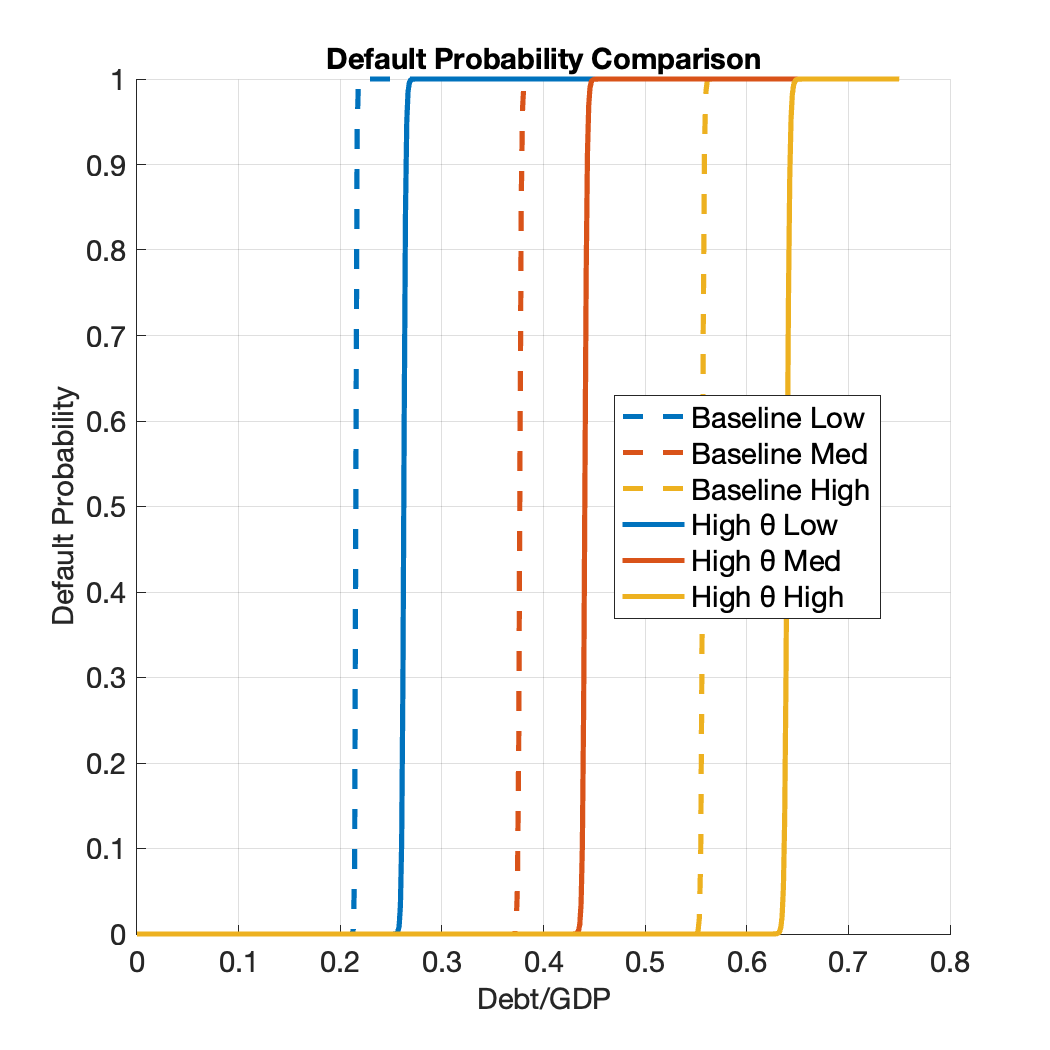
\includegraphics[width=\linewidth]{default_prob_comparison.png}\\[0.3em]
    {\scriptsize Default probabilities}
  \end{columns}
  \vspace{0.3em}
  {\scriptsize Single-crossing pivot around $B^*(y)$; PRO discounts safe region and softens near-doom.}
\end{frame}

\begin{frame}{Impulse Responses: Transitory Shock}
  \begin{columns}[T,onlytextwidth]
    \column{0.5\textwidth}
    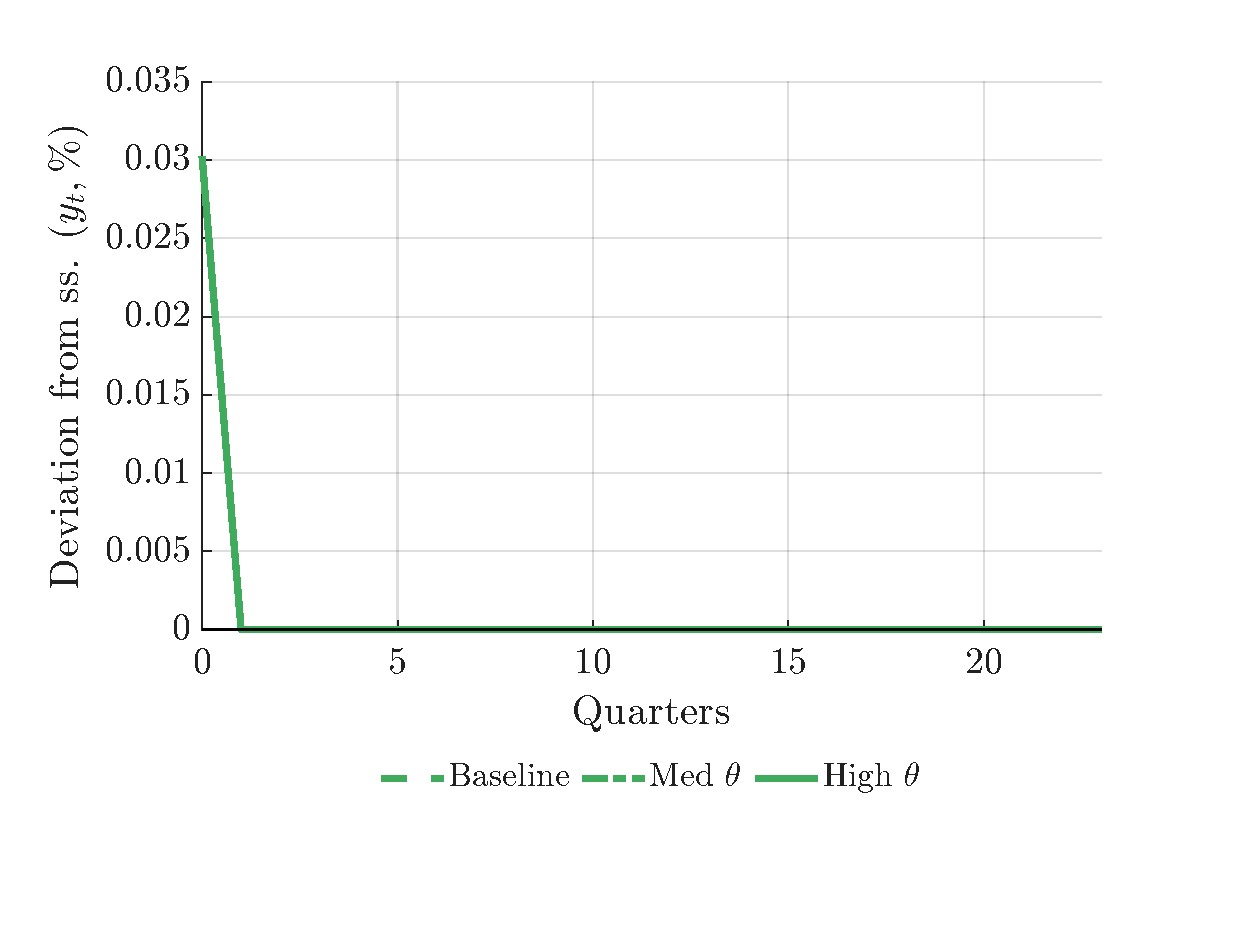
\includegraphics[width=\linewidth]{comparison_figure_13.pdf}\\[-0.5em]
    {\scriptsize Output}
    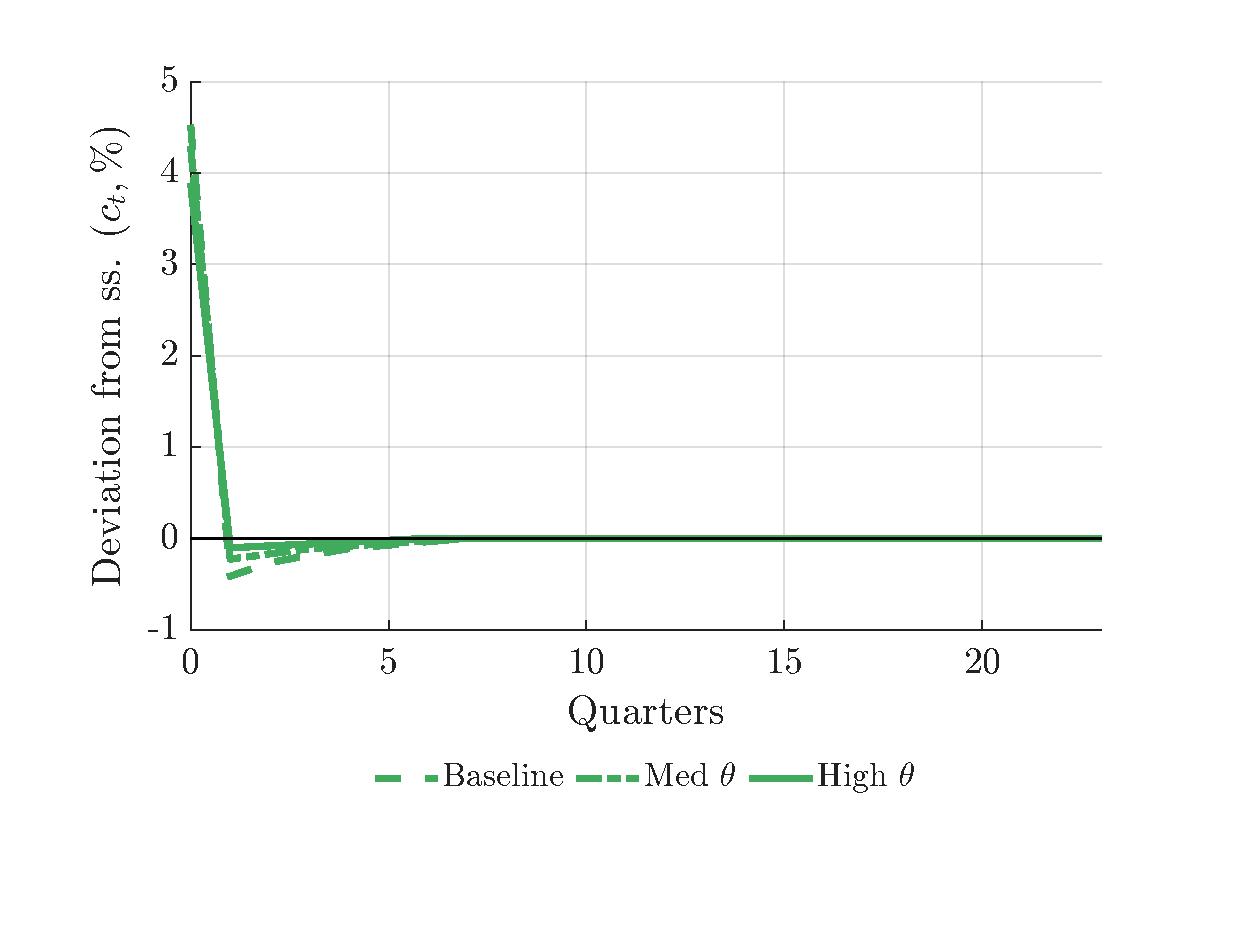
\includegraphics[width=\linewidth]{comparison_figure_15.pdf}\\[-0.5em]
    {\scriptsize Consumption}
    \column{0.5\textwidth}
    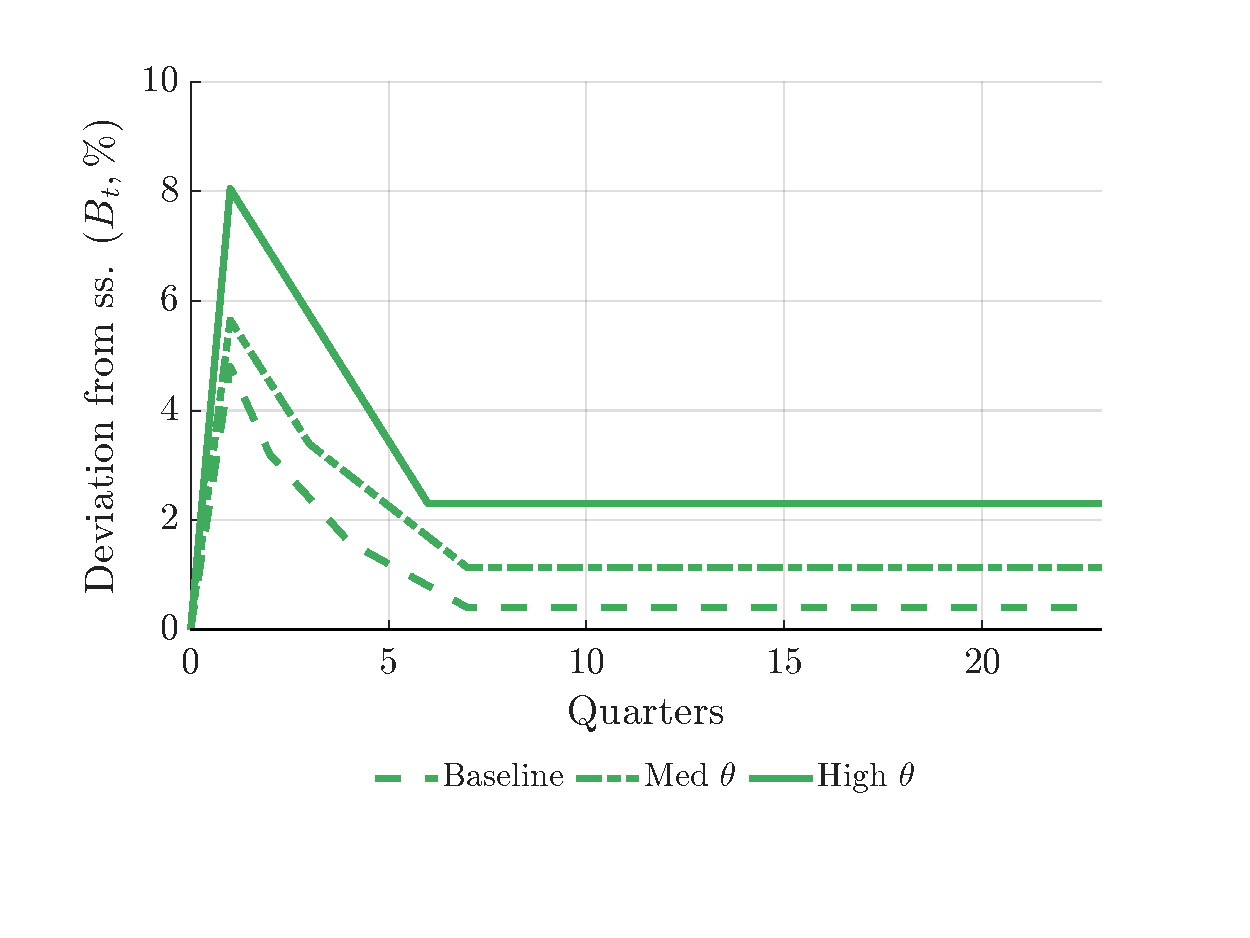
\includegraphics[width=\linewidth]{comparison_figure_14.pdf}\\[-0.5em]
    {\scriptsize Debt}
    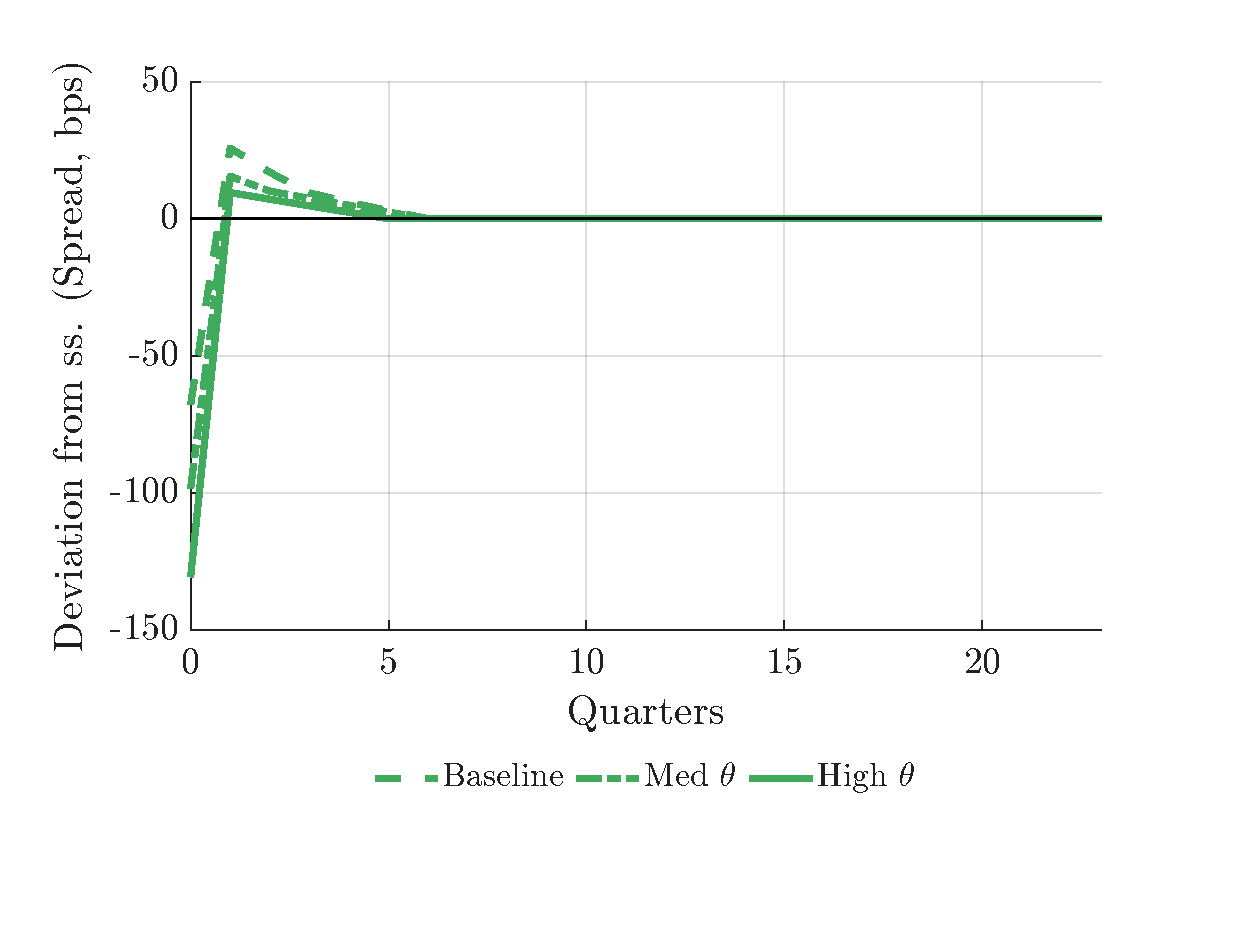
\includegraphics[width=\linewidth]{comparison_figure_16.pdf}\\[-0.5em]
    {\scriptsize Spread}
  \end{columns}
\end{frame}

\begin{frame}{Impulse Responses: Persistent Shock}
  \begin{columns}[T,onlytextwidth]
    \column{0.5\textwidth}
    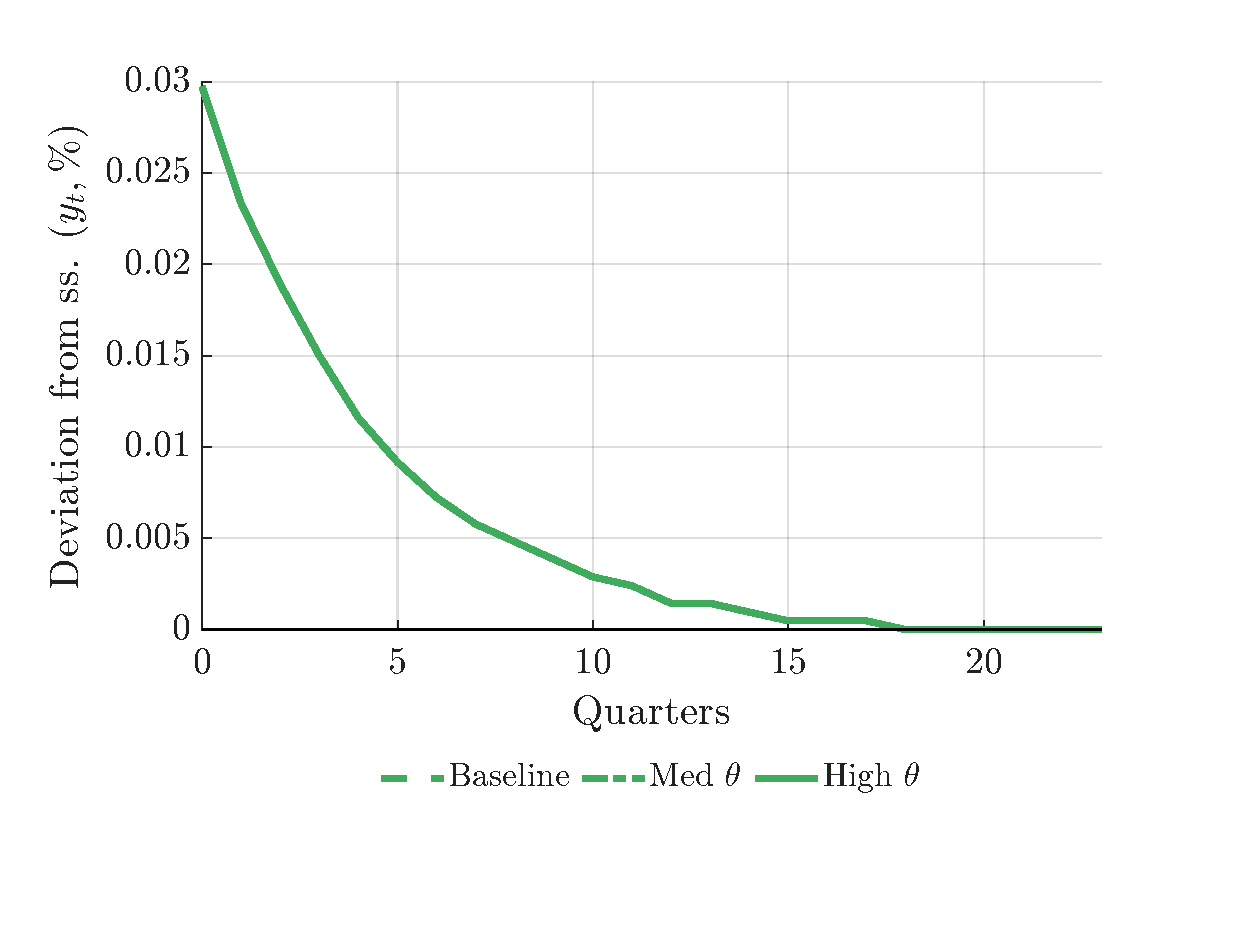
\includegraphics[width=\linewidth]{comparison_figure_17.pdf}\\[-0.5em]
    {\scriptsize Output}
    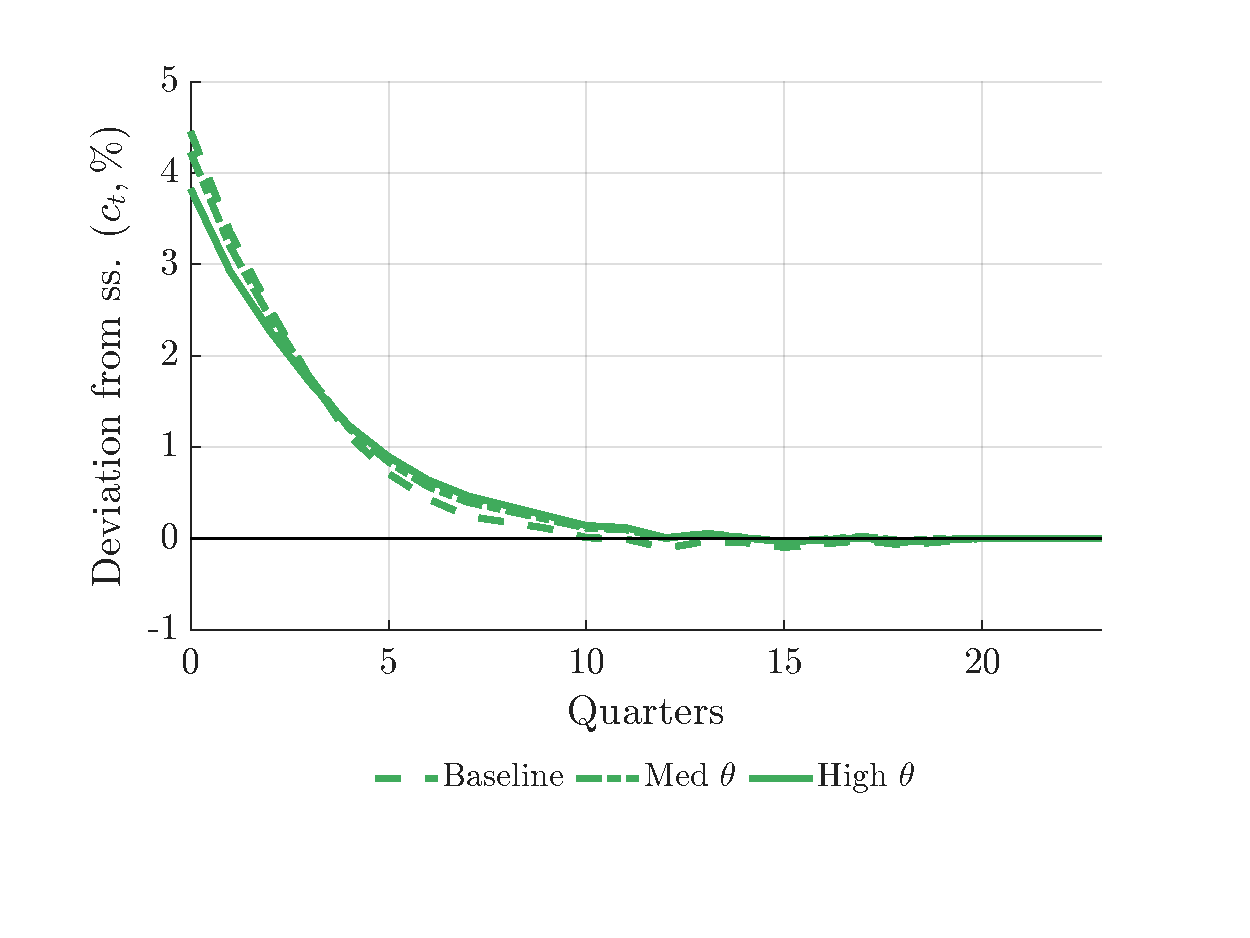
\includegraphics[width=\linewidth]{comparison_figure_19.pdf}\\[-0.5em]
    {\scriptsize Consumption}
    \column{0.5\textwidth}
    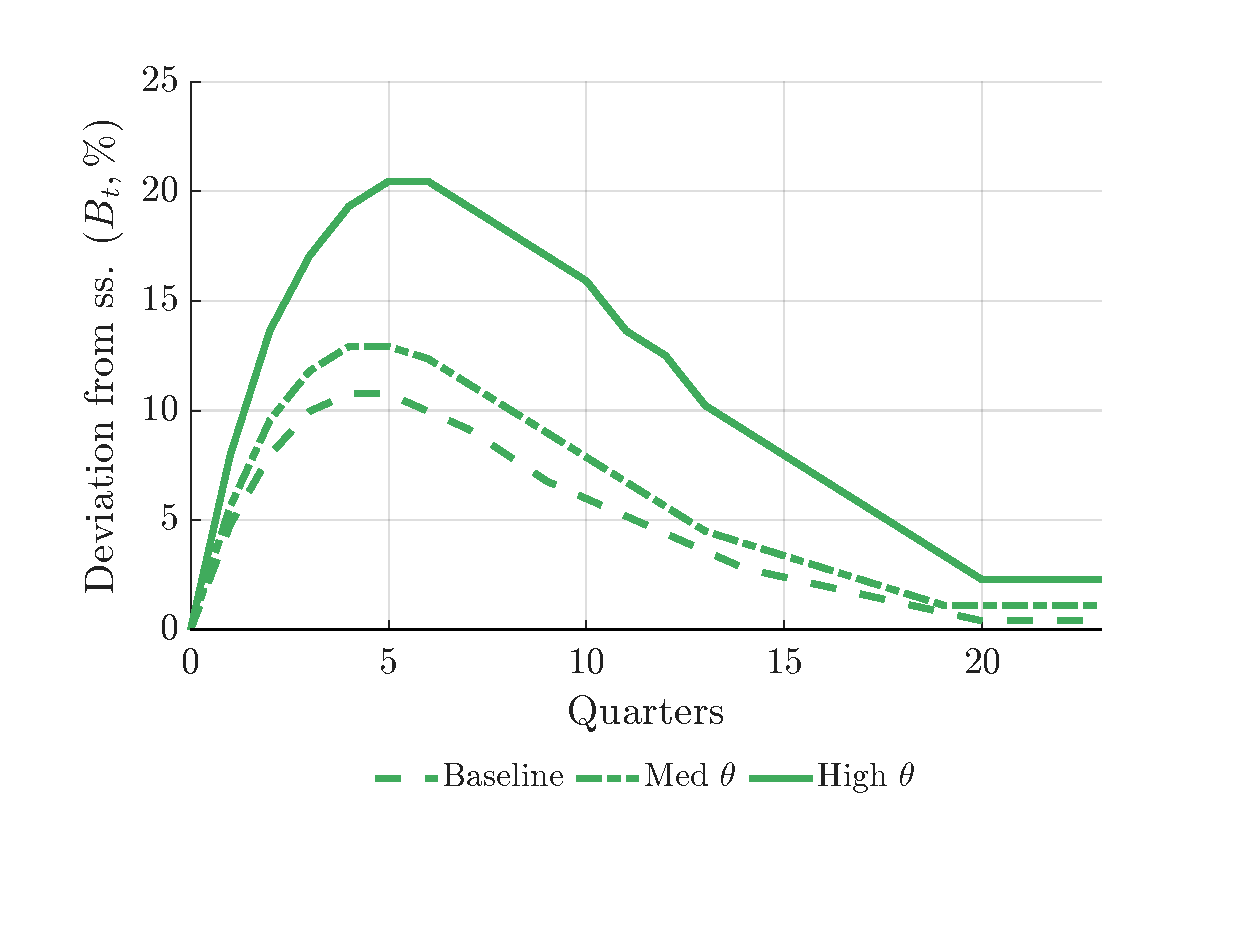
\includegraphics[width=\linewidth]{comparison_figure_18.pdf}\\[-0.5em]
    {\scriptsize Debt}
    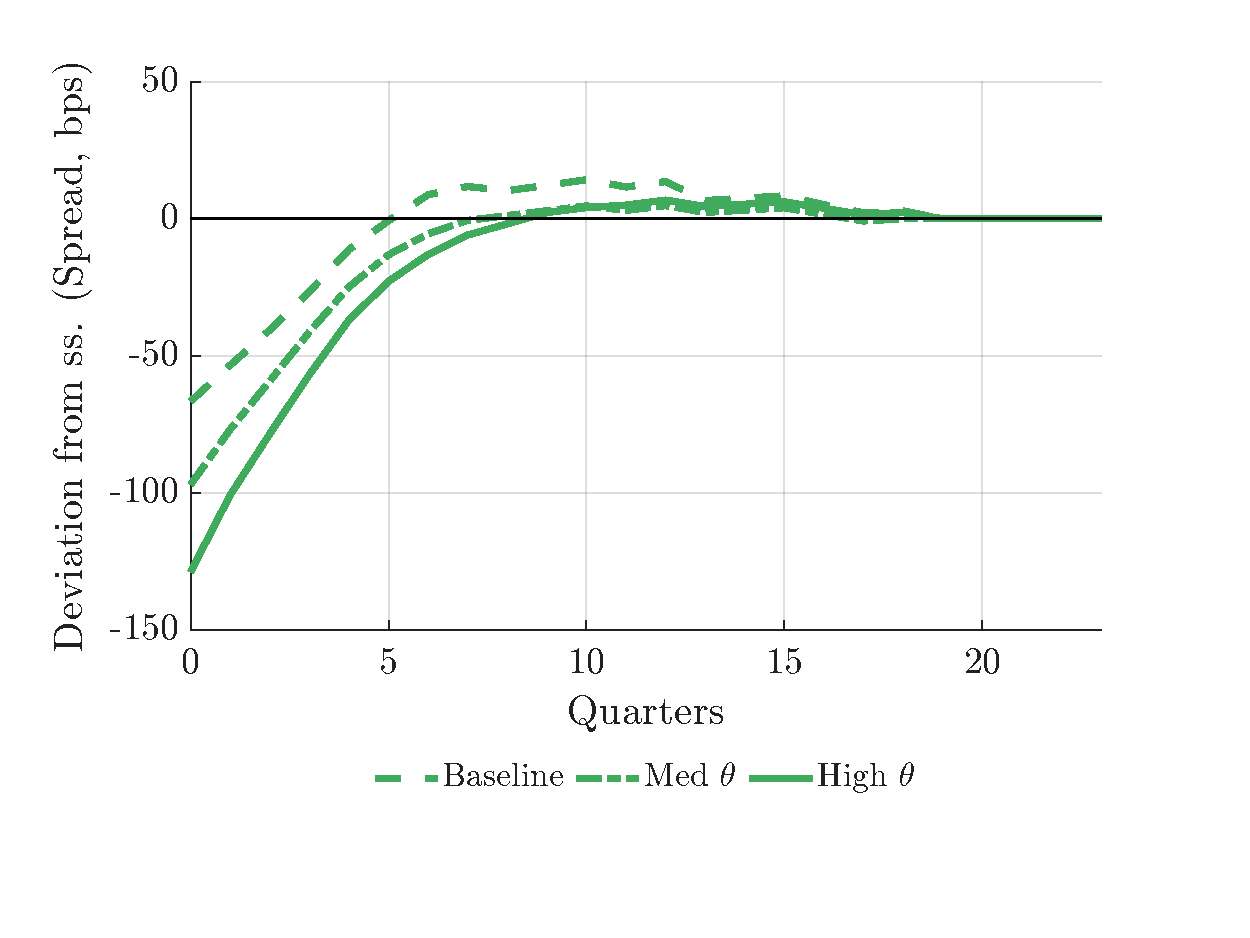
\includegraphics[width=\linewidth]{comparison_figure_20.pdf}\\[-0.5em]
    {\scriptsize Spread}
  \end{columns}
\end{frame}

% Microfoundation
\section{Microfoundation (RI)}

\begin{frame}{Rational Inattention: Tail Weight from Attention}
  \begin{itemize}
    \item Lenders choose precisions $(a_\mu,a_\sigma)$ at convex cost
          $\Phi(a_\mu,a_\sigma)$.
    \item Closed-form linear map: $\displaystyle
            \theta_{\mathrm{RI}}(y,B')=\min\Big\{\,1+\frac{\varphi^2}{\kappa_\sigma}\,\mathcal
            S(y,B')\,,\;\bar\theta\,\Big\}$.
    \item Pricing remains the same operator evaluated at $\theta_{\mathrm{RI}}(\cdot)$;
          comparative statics inherit.
  \end{itemize}
  \vspace{0.5em}
  \begin{equation*}
    q(B',y)=\mathcal T_{\theta_{\mathrm{RI}}(y,B')}[q](B',y),\qquad \mathcal S=\E\Big[\partial U/\partial\theta\Big]\ge0.
  \end{equation*}
\end{frame}

\begin{frame}{Empirical Hook: Misreporting \texorpdfstring{$\Rightarrow$}{=>} Higher Dispersion Attention}
  \begin{itemize}
    \item Degraded mean-information ($a_\mu$) raises marginal value of dispersion info
          $\mathcal S$.
    \item $\uparrow\mathcal S\Rightarrow \uparrow a_\sigma\Rightarrow \uparrow \theta_{\mathrm{RI}}$: higher average spreads, steeper pivot, decoupling.
  \end{itemize}
\end{frame}

% Policy and information
\section{Policy \& Information}

\begin{frame}{Ramsey with PRO: Transfers Cannot Undo Price Wedge}
  \begin{gather*}
    c_t+\kappa B_t+\tau_t = y_t+\big(B_{t+1}-(1{-}\delta)B_t\big)\,q_\theta(y_t,B_{t+1}),\\
    \E_0\sum_t \beta^t\tau_t=0,\quad u'(\cdot)>0,\ u''(\cdot)<0.
  \end{gather*}
  \begin{itemize}
    \item Intertemporal trade price distorted by PRO persists in implementability; wedge
          creates deadweight loss.
    \item Result: $W^R_\theta<W^R_1$ even with optimal transfers.
  \end{itemize}
\end{frame}

\begin{frame}{Endogenous Beliefs and Transparency}
  Belief dynamics with negativity bias:
  \begin{gather*}
    \theta_{t+1}=\lambda\,\theta_t+(1{-}\lambda)\,\widehat\theta(\{d_s\}),\quad
    \xi(y,B)=\max\Big\{0,\tfrac{P_1-P_{\theta_t}}{P_1}\Big\},\quad \text{defaults move beliefs more}.
  \end{gather*}
  Effective transparency:
  \begin{gather*}
    \theta_{\mathrm{eff}}(\alpha,\theta)=\alpha\cdot 1+(1{-}\alpha)\cdot\theta,\qquad
    \alpha^*:\ \frac{\mathrm d}{\mathrm d\alpha}W(\alpha)=\gamma\alpha.
  \end{gather*}
  \begin{itemize}
    \item Persistent PRO in invariant beliefs; optimal transparency rises with PRO
          severity.
  \end{itemize}
\end{frame}

% Computation
\section{Computation}

\begin{frame}{Computation and Stability}
  \begin{itemize}
    \item Value and price iteration on $(N_y{=}201, N_B{=}600)$ grid; OpenMP parallel.
    \item Stabilized log-sum-exp for borrowing/default logits; infeasible-consumption
          guard.
    \item Convergence tolerances $10^{-6}$; long simulation for moments and IRFs.
  \end{itemize}
  \vspace{0.5em}
  \centering
  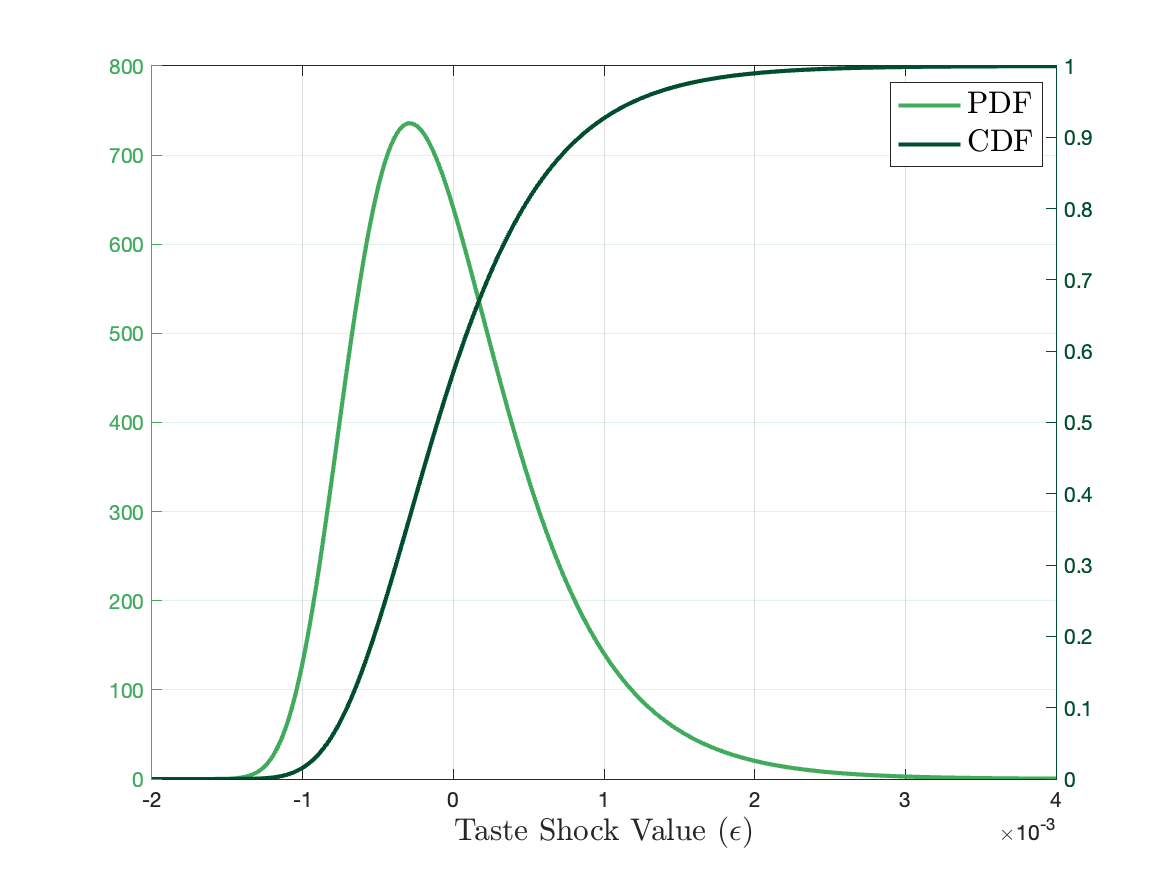
\includegraphics[width=0.6\linewidth]{gumbel_distribution.png}
  \\
  {\scriptsize Mean-zero Gumbel: logit and LSE arise naturally}
\end{frame}

% Conclusion
\section{Conclusion}

\begin{frame}{Takeaways}
  \begin{itemize}
    \item Single operator with PRO produces a \emph{pivot} in price/spread schedules.
    \item Sovereigns deleverage yet face higher average spreads; volatility falls
          (stability illusion).
    \item RI microfoundation endogenizes the tail tilt; policy/info extensions clarify
          limits and levers.
    \item Event hooks (Argentina) align with pivot, threshold, and decoupling
          predictions.
  \end{itemize}
\end{frame}

% Backup (optional)
\appendix
\section{Backup}

\begin{frame}{Operator View (Sketch)}
  \begin{itemize}
    \item $\mathcal T_\theta$ is positive and order-preserving; fixed point unique under slope condition.
    \item Fixed-point differentiation signs $\partial_\theta q_\theta$; monotone
          propagation yields pivot.
  \end{itemize}
\end{frame}

\end{document}

